\documentclass[12pt]{examdesign}
\usepackage[spanish]{babel}
\OneKey
\usepackage[utf8]{inputenc}
\usepackage[T1]{fontenc}
\usepackage{amsmath}
\usepackage{pifont}
%-----------------------------------------------------------------------------------------------
%\usepackage{gfsartemisia-euler}
\usepackage{graphicx}
\usepackage{float}
\usepackage{amscd}
\usepackage{amsfonts}
\usepackage{amssymb}
\usepackage{mathtools}
\usepackage{amsthm}
\usepackage[all]{xy}
\usepackage{enumitem}
\usepackage{multicol}
\usepackage{verbatim}
\usepackage[colorlinks=true,
breaklinks=true,
linkcolor=blue,
urlcolor=red,
bookmarksopen=true]{hyperref}
\usepackage[pdftex,dvipsnames]{xcolor}
\definecolor{aqua}{rgb}{0.0, 1.0, 1.0}
\definecolor{caribbeangreen}{rgb}{0.0, 0.8, 0.6}
\definecolor{tealgreen}{rgb}{0.0, 0.51, 0.5}
\definecolor{upforestgreen}{rgb}{0.0, 0.27, 0.13}
\definecolor{napiergreen}{rgb}{0.16, 0.5, 0.0}
\definecolor{capri}{rgb}{0.0, 0.75, 1.0}
\definecolor{calpolypomonagreen}{rgb}{0.12, 0.3, 0.17}
\definecolor{azure(colorwheel)}{rgb}{0.0, 0.5, 1.0}
\definecolor{dukeblue}{rgb}{0.0, 0.0, 0.61}
\definecolor{bole}{rgb}{0.47, 0.27, 0.23}
\definecolor{gris}{gray}{0.975}
%----------------------------------------------------------------------------------------------
% Si desea utilizar \@@line para definir su propio encabezado de examen o palabras del encabezado, 
% asegúrese de usar \makeatletter y \makeatother en los lugares apropiados, de lo contrario 
% podría obtener errores.
%-----------------------------------------------------------------------------------------------
\theoremstyle{plain}
\newtheorem{theorem}{Theorem}[section]
\newtheorem{thm}[theorem]{Teorema}
\newtheorem{cor}[theorem]{Corolario}
\newtheorem{lem}[theorem]{Lema}
\newtheorem{pro}[theorem]{Proposición}
\newtheorem{axs}[theorem]{Axiomas}
\newtheorem{axi}[theorem]{Axioma}
\theoremstyle{definition}
\newtheorem{exas}[theorem]{Ejemplos}
\newtheorem{exa}[theorem]{Ejemplo}
\newtheorem{defi}[theorem]{Definición}
\theoremstyle{remark}
\newtheorem{rmk}[theorem]{Observación}
\newtheorem{step}{Step}
\newtheorem{xca}[theorem]{Ejercicio}
\newtheorem{prob}[theorem]{Pregunta}
\newtheorem{rmks}[theorem]{Observaciones}
\newtheorem*{proofmt}{Prueba del Teorema Principal}
\usepackage[centerlast,small,sc]{caption}
\setlength{\captionmargin}{20pt}
\newcommand{\axref}[1]{Axioma~\ref{#1}}
\newcommand{\defref}[1]{\textbf{Definición}~\ref{#1}}
\newcommand{\coref}[1]{\textbf{Corolario}~\ref{#1}}
\newcommand{\thref}[1]{\textbf{Teorema}~\ref{#1}}
\newcommand{\lref}[1]{\textbf{Lema}~\ref{#1}}
\newcommand{\exaref}[1]{Ejemplo~\ref{#1}}
\newcommand{\xcaref}[1]{Ejercicio~\ref{#1}}
\newcommand{\rmkref}[1]{Observación~\ref{#1}}
\newcommand{\pref}[1]{\textbf{Proposición}~\ref{#1}}
\newcommand{\fref}[1]{Figura~\ref{#1}}
\newcommand{\tref}[1]{Tabla~\ref{#1}}
\newcommand{\cref}[1]{\textbf{Capítulo}~\ref{#1}}
\newcommand{\sref}[1]{\textbf{Sección}~\ref{#1}}
\newcommand{\aref}[1]{Apéndice~\ref{#1}}
\newcommand{\eref}[1]{Ecuación~\eqref{#1}}
\newcommand{\dref}[1]{Diagrama~\eqref{#1}}
\usepackage{makeidx}
\usepackage{tikz,tkz-tab}%
\usetikzlibrary{matrix,arrows,positioning,shadows,shadings,backgrounds,
	calc, shapes, tikzmark}
\usepackage{tcolorbox, empheq}%
\tcbuselibrary{skins,breakable,listings,theorems}

\tcbset{opteqC/.style={skin=beamer,colback=red!1!white}}
\newcommand{\celda}[2]{
	\begin{minipage}{#1mm}
		\centering
		\vspace{2mm}
		#2
		\vspace{2mm}
	\end{minipage}
}
\makeatletter
\begin{examtop}
	\@@line{\parbox{3in}{\classdata \\[0.5cm]
			\textcolor{upforestgreen}{\textbf{\underline{T.P.N$^\circ$}}~\fbox{\textsc{7}}} \examtype}
		%                  ^^^^^^
		\hfill
		\parbox{3in}{\normalsize \namedata}}
	\bigskip
\end{examtop}

\def\namedata{\textcolor{upforestgreen}{\textbf{Estudiante}}:\hrulefill \\[\namedata@vspace]
	\textcolor{upforestgreen}{\textbf{Curso y División}}: 2do año, IV-VI \\[\namedata@vspace]
	\textcolor{upforestgreen}{\textbf{Profesor}}: Ferreira, Juan David \\[\namedata@vspace]
	\textcolor{upforestgreen}{\textbf{Fecha de Entrega}}:\hrulefill}
% manual page 11        
\begin{keytop}%
	\@@line{\hfill \Huge\texttt{\textcolor{upforestgreen}{Respuestas 
				Trabajo Práctico N$^\circ$~\fbox{\textsc{7}}}} \hfill}
	\bigskip
\end{keytop}%
\makeatother
\examname{\textcolor{upforestgreen}{\underline{\textbf{Potenciación-Radicación.}}}}

\SectionPrefix{\textcolor{upforestgreen}{\textbf{Sección \arabic{sectionindex}}.} \space}
\Fullpages
\ContinuousNumbering
\DefineAnswerWrapper{}{}
\NumberOfVersions{1}
\class{{\textcolor{upforestgreen}{\large\textbf{E.P.E.S. Nro 51 ``J. G. A.''}}\\[0.5cm]
		\textcolor{upforestgreen}{{\large \textbf{Matemática}}}}}
\usepackage{scalerel,amssymb}
\def\mcirc{\mathbin{\scalerel*{\circ}{j}}}
\def\msquare{\mathord{\scalerel*{\Box}{gX}}}

\begin{document}
	%-------------------------------             SHORT ANSWER        ------------------------%
	\begin{fillin}[title={Leemos el material de consulta y realizamos las actividades propuestas}]
		
		\begin{question}
			Completa las siguientes potencias y respeta la regla de los signos en la multiplicación con enteros:
			\begin{enumerate}
				\item La potencia menos diez al \underline{cuadrado} es $(-10)^{2}=$\underline{$100$}.
				\item La potencia menos dos a la \blank{quinta} es $(-2)^{5}=$\blank{$-32$}.
				\item La potencia tres a la \blank{quinta} es $(3)^{5}=$\blank{$243$}.
				\item La potencia menos cuatro al \blank{cubo} es $(-4)^{3}=$\blank{$-64$}.
				\item La potencia menos cinco a la \blank{cuarta} es $(-5)^{4}=$\blank{$625$}.
				\item La potencia menos dos a la \blank{sexta} es $(-2)^{6}=$\blank{$64$}.
			\end{enumerate}
		\end{question}
	    \begin{question}
	    	Colocar ``$<$'' , ``$>$'' ó ``$=$'' según corresponda en cada caso:
	    	\begin{enumerate}
	    		\item $(-2)^4$ \blank{ $>$ } $(-2)^{5}$.
	    		\item $(-3)^2$ \blank{ $>$ } $(-2)^{3}$.
	    		\item $(-2)^4$ \blank{ $=$ } $(-4)^{2}$.
	    		\item $(-9)^0$ \blank{ $>$ } $9^{0}$.
	    		\item $\sqrt[]{144}$ \blank{ $<$ } $(-4)^{2}$.
	    		\item $\sqrt[3]{-64}$ \blank{ $=$ } $(-4)^{1}$.
	    		\item $(-3)^{2}$ \blank{ $<$ } $(-4)^{2}$.
	    		\item $(-7)^0$ \blank{ $>$ } $(-1)^{7}$.
	    		\item $\sqrt[3]{-27}$ \blank{ $<$ } $\sqrt[3]{-8}$
	    	\end{enumerate}
	    \end{question}
    \end{fillin}
	%--------------------------------------------------------------------------------%
	\begin{endmatter}
		\vspace{.2cm}
		\centerline{\large \textcolor{upforestgreen}{\textbf{Potenciación y Radicación en El Conjunto de los Números Enteros ${\mathbb Z}$}}}
		\vspace{.2cm}
		\begin{tcolorbox}[colback=red!10!white, colframe=tealgreen, title=\textbf{Material de consulta}]
			\begin{defi}[Potenciación]
					La potenciación es una operación que abrevia una multiplicación de factores iguales
				\begin{align*}
				2^{1} &= 2,\mbox{ dende se lee ``dos a la uno''},\\
				2^{2} &= 2\cdot 2=4,\mbox{ donde se lee ``dos al cuadrado'' },\\
				2^{3} &= 2\cdot 2\cdot 2=8,\mbox{ donde se lee ``dos al cubo'' },\\
				2^{4} &= 2\cdot 2\cdot 2\cdot 2=16,\mbox{ donde se lee ``dos a la cuarta''},\\
				2^{5} &= 2\cdot 2\cdot 2\cdot 2\cdot 2=32,\mbox{ donde se lee ``dos a la quinta''},\\
				\vdots&\;\vdots
				\end{align*}
				Además cualquier número (distinto de cero) elevado a la cero es 1 y 1 elevado a cualquier exponente es 1. 
			\end{defi}
		\end{tcolorbox}
		\vspace{.2cm}
		
		Si tomamos el último ejemplo, podemos describir los elementos de la potenciación, que son los siguientes:
		
		\begin{center}
			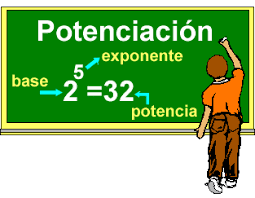
\includegraphics[width=10cm, height=5cm]{descarga.png}
		\end{center} 
		El \textbf{exponente} es el número que indica la cantidad de veces que debe multiplicarse la \textbf{base} por sí misma, y el resultado se llama \textbf{Potencia}.
		\vspace{.2cm}
		\begin{tcolorbox}[opteqC]
			\begin{exa}
				Siguiendo el concepto de Potencia en el conjunto de los Números Enteros, se tiene que: ``Si el exponente es par, la potencia lleva signo positivo. Si el exponente es impar, la potencia lleva el signo de la base''
				
				\begin{align*}
				2^{3} &=2\cdot 2\cdot 2=8&y&& (-2)^{4}&=(-2)\cdot(-2)\cdot(-2)\cdot(-2)=16\\
				(-5)^{3} &= (-5)\cdot(-5)\cdot(-5)=-125&y&& (-10)^{2}&=(-10)\cdot(-10)=100\\
				(-3)^{3} &=(-3)\cdot(-3)\cdot(-3)=-27&y&& (-12)^{2} &= (-12)\cdot(-12)=144
				\end{align*}
			\end{exa}
		\end{tcolorbox}
		\vspace{.2cm}
		Intentamos completar cuando sea posible
		\begin{align*}
		\msquare^{2} &=49&\msquare^{2} &=25 &\msquare^{3} &=81&\msquare^{6} &=64
		\end{align*}
		\begin{tcolorbox}[colback=red!10!white, colframe=tealgreen, title=\textbf{Material de consulta}]
			\begin{defi}[Radicación]
				La Radicación es una operación que relaciona de manera inversa a la Potenciación.
				\begin{center}
					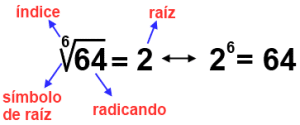
\includegraphics[width=6cm, height=3cm]{images.png}
				\end{center}
				\begin{align*}
				\sqrt[2]{9}&=3,\mbox{ porque $3^{2}=9$ dende se lee ``raíz cuadrada de 9 es igaul a 3''},\\
				\sqrt[2]{9}&=\sqrt[]{9}=3,\mbox{ porque cuando el índice es 2 (dos) se puede omitir escribirlo.},\\
				\sqrt[3]{125}&=5,\mbox{ porque $5^{3}=125$, donde se lee ``raíz cúbica de 125 es igual a 5''},\\
				\sqrt[4]{81}&=3,\mbox{ porque $3^{4}=81$ donde se lee ``raíz cuart de 81 es igual a 3''},\\
				\vdots&\;\vdots
				\end{align*} 
			\end{defi}
		\end{tcolorbox}
		\vspace{.2cm}
		
		\begin{tcolorbox}[opteqC]
			\begin{exa}
				Siguiendo el concepto de Radicación en el conjunto de los Números Enteros, se tiene que: ``Si el \textcolor{red}{índice} es \textbf{impar}, la raíz lleva signo del \textbf{radicando}. Si el \textcolor{red}{índice}e es \textbf{par} la raíz tiene solución si el radicando es \textbf{positivo}''
				
				A modo de ejemplo, calculamos si es posible (sin usar la calculadora), las siguientes raíces:
				\begin{align*}
				\sqrt[3]{121}&=\dots\dots,&\sqrt[4]{-16}&=\dots\dots,&
				\sqrt[]{100}&=\dots\dots,&\sqrt[3]{-8}&=\dots\dots
				\end{align*}
			\end{exa}
		\end{tcolorbox}
	
		
	\end{endmatter}
\end{document}